\documentclass{article}

\pdfpagewidth 8.5in
\pdfpageheight 11in

% \setlength\topmargin{0in}
% \setlength\headheight{0in}
% \setlength\headsep{0in}
% \setlength\textheight{7.7in}
\setlength\textwidth{6.5in}
\setlength\oddsidemargin{0in}
\setlength\evensidemargin{0in}
% \setlength\parindent{0.25in}
% \setlength\parskip{0.25in} 

\usepackage{makeidx}
\makeindex
\usepackage[dvips]{graphicx}

\usepackage{url}

\pagestyle{headings}

\author{Geoff Lawler \url{<geoff.lawler@cobham.com>} \and {Michael Elkins \url{<michael.elkins@cobham.com>}}}

\title{Watcher User's Guide}

\begin{document}
\maketitle
\newpage 

\tableofcontents
\newpage

\section{Introduction}

The {\it watcher}, or {\it watcher system} allows users to visualize emulated Mobile As-Hoc Networks. 

\section{General Watcher Information}
\subsection{Watcher Architecture, Communications, and Component Interactions}

\begin{figure}[htb]
\centering
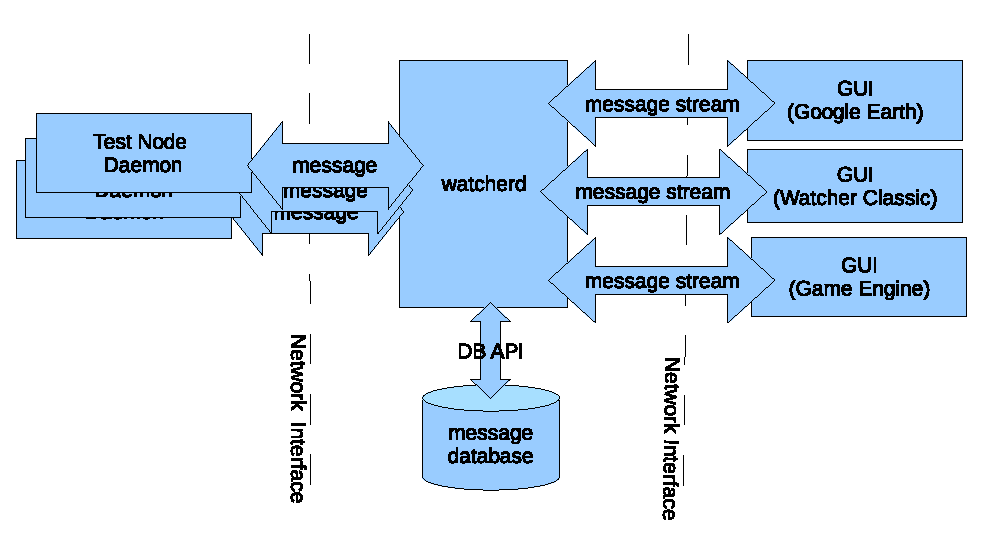
\includegraphics[width=0.8\textwidth]{watcherArch.eps}
\caption{The basic architecture of the watcher system.}
\label{fig:watcherArch}
\end{figure}

Figure \ref{fig:watcherArch} shows the three main components in the watcher system: test node daemons (or ``feeders''), a watcher
daemon, and a number of graphical user interfaces (or ``GUIs''). The basic operation is this: the test nodes feed state 
information to a running instance of the watcher daemon, {\it watcherd}. The watcher daemon saves all the state information
locally to a database. A GUI connects to a running watcher daemon and requests a stream of state information, then displays it
using some (most likely) graphical mechanism. The daemon acts as a message cache and demulitplexer, streaming multiple
message streams from multiple test nodes into a single stream of messages. 

The interface between the watcher daemon and the test node is a simple message interface. The test node daemon connects
to a daemon, sends one or more messages, then disconnects. Some messages contain abstract state information about that test node
such as current set of neighbors, current location, etc. Other messages contain lower-level graphical display commands like ``change
color'' or ``draw an edge between these two nodes''.  For a list of all supported message, see the {\it watcher::event::Message} class 
in the watcher developer documentation. 

The interface between the GUI(s) and the watcher daemon is also message based, but also includes the concept of a message
stream. The stream is composed of messages and has an interface that manipulates the stream content, time, direction, and rate. A message
stream can start at any time {\it t} for which there is data. The stream rate can be set as a multiplier of real time. For instance
a GUI can request that the stream go 10x the speed at which the messages were received. (This only will work of course if there is 
a cache of messages that can be sent at 10x - once the message cache is exhausted, the stream is sent at the rate the messages
are received, 1x real time.) The concept of manipulating a message stream by rate and time allows GUIs to act as test bed "TiVO"s, playing 
back an arbitrary stream of test node data in reverse, forward, jumping around the stream as the user requests. 

Depending on which components are running and how they are started, the watcher system can be said to be running in different modes: a ``live'' mode, 
a ``playback'' mode, and a ``record'' mode. In all modes, a {\it watcherd} instance must be running.  These modes
can be moved into and out of in real time depending on the needs of the user. In record mode, the test nodes and a watcher daemon are
run. The test nodes send state data to the daemon, the the daemon writes those messages to a local database. In live mode, the test 
nodes are feeding data to the daemon (which writes the information to a database) and some number of GUIs connect to the 
daemon and request a message stream. Note that the GUIs can request messages from the start of the test run - they are not
constrained to ``live'' messages; live mode simply means that there are, at that moment, new messages arriving at the daemon
and being recorded. The last mode is playback mode and does not involve test node daemons. In this mode, the watcher daemon
is started with an existing database full of messages and it just waits for connections from a GUI. When a GUI connects, the 
watcher daemon streams it the requested messages, this ``playing back'' a ``recorded'' test run. 

\subsection{Obtaining and Building Watcher}
\subsubsection{Obtaining}
The watcher is GPL'd software although it is not currently public-ally available. This will change in the near future. Future versions of this 
document will be updated after the watcher is public-ally released giving the download location. In the meantime please contact the authors 
of this document to obtain instructions on getting the watcher. 

The watcher system is written in C++. 

\subsubsection{Repository Structure}
The watcher system uses the GNU auto-tools build system for most components. (GUIs are an exception as the GUI libraries used, generally have 
their own build systems, qmake for QT, etc).  The source code for all watcher components is in .\slash src. The basic layout of the source tree is given
below. Note that only the ``important'' directories are listed to minimize clutter. 

\begin{description}
\item[.\slash src] Holds all watcher system source code. 
\begin{description}
\item[.\slash src\slash clients] Anything that is a client of the watcher daemon, including GUIs and test node daemons, is in here. 
\item[.\slash src\slash doc] Holds the \LaTeX{} code for generating Doxygen based watcher documentation including the Watcher User's Guide.
\item[.\slash src\slash idsCommunications] Holds the code for building the (optional) hierarchy communications library which the watcher uses to talk to hierarchy software running on the test nodes. 
See section \ref{watcherHierarchyClient} for details.
\item[.\slash src\slash libwatcher] Holds the source code for two libraries used in the watcher system: libwatcher, which is a generic communications mechanism used by watcher components
to talk to one another, and libwatchermessage, which contains the code for all watcher messages and a mechanism to parse them. 
\item[.\slash src\slash logger] The code the watcher system uses for logging. This is a small wrapper around calls to log4cxx, a standard logging library from the good people at Apache. 
\item[.\slash src\slash util] Code for a utility library used by some watcher components. 
\item[.\slash src\slash watcherd] The code for the watcher daemon, {\it watcherd}. 
\end{description}
\item[.\slash doc] Watcher documentation, including basic architecture documents and the location where the Doxygen generated developer's guide is when it is built. 
\begin{description}
\item[.\slash doc\slash html] The html based developer's guide. (Must be built - \vbox{{\tt make -C .\slash src doc}} to do so.)
\item[.\slash doc\slash man] If configured, this is the location of the man pages built by \vbox{{\tt make -C .\slash src doc}}.
\item[.\slash doc\slash latex] If configured, this is the location of the latex-based developer's guide built by 
\vbox{{\tt make -C ./src doc}}.
\end{description}
\item[.\slash tars] Some source code (tar'd up) for third party libraries used by the watcher system including {\bf log4cxx} (and its required libraries \bf{apr} and
\bf{apr-util}), \bf{libconfig}, \bf{libidmef}, and \bf{libqwt}. 
\end{description}

\subsubsection{Dependencies}
The watcher system has the following dependencies:
\begin{description}
\item[Third Party] Watcher uses a number of third party libraries. 
\begin{description}
\item[sqlite 3] The watcher daemon uses sqllite for all database operations. 
\item[libconfig 1.3.1] The system uses this for creating, reading, and writing to configuration ("cfg") files. 
\item[log4cxx 0.10.0] (This depends on lib apr 1.3.3 and lib apr util 1.3.4). This is used for all logging in the watcher.  It is a clone of Java's log4j logging package. 
\item[boost 1.38] The watcher makes extensive use of Boost. This C++ library used more many things: serialization, network code, regular expressions, etc. 
\item[Legacy Watcher] The ``legacy watcher'' is the Qt\slash OpenGL based GUI. If not building the legacy watcher, these libraries are not needed. 
\begin{description}
\item[Qt 4.3] Qt is used by the legacy watcher to supply the GUI widgets (windows, frames, menus, buttons, etc) and to wrap the OpenGL which displays the MANET. If not building the legacy watcher, 
    Qt is not needed. 
\item[qwt-5.1.1] A small Qt-based library used to draw the 2d scrolling graphs in the legacy watcher. If not building the legacy watcher, Qwt is not needed.
\end{description}
\item[OGRE Watcher] The OGRE watcher is an OGRE-based GUI. If not building the OGRE watcher GUI, these libraries are not needed. 
\begin{description}
\item[OGRE] The ogreWatcher uses the Object-Oriented Graphics Rendering Engine (OGRE) for graphics. 
\item[OIS] The ogreWatcher uses the Object Oriented Input System (OIS) for mouse and keyboard input. 
\item[CEGUI] The ogreWatcher uses Crazy Eddie's Graphical User Interface (CEGUI) for GUI widgets. 
\end{description}
\item[Watcher3D] The Delta-3D based watcher GUI. If not building the watcher3d, these libraries are not needed. 
\begin{description}
\item[delta 3d] Delta 3d is used for graphics rendering in watcher3d. 
\end{description}
\end{description}
\item[Internal] These are the libraries that watcher uses internally. 
\begin{description}
\item[libwatcherutil] Holds a few things that most components need, like parsing command line args to get to the cfg file.
\item[liblogger] A small wrapper around log4cxx to abstract which logging library we use. 
\item[libwatcher] The core of the watcher messaging system, the watcher APIs between test node daemons, a watcher daemon, and the GUI(s)s.
\end{description}
\end{description}

\subsubsection{Building}

First make sure that the dependencies above are built and installed on the build machine. For most dependencies you can use the package management system to install 
the dependencies. For example, on Fedora 11, the command {\tt yum install boost-devel boost qt qt-devel log4cxx log4cxx-devel libconfig libconfig-devel ...} will install the 
required dependencies. Some libraries may not be widely available (like libidmef), in these cases check in the {\tt tars} directory. The source code may be there. 

Once the required dependencies are installed, build the core watcher components (libwatcher, watcherd, and test node binaries). These are auto-tools based. It should be as easy 
as the canonical. It should be as easy as the canonical {\tt .\slash configure \&\& make \&\& sudo make install}. (If .\slash configure does not exist, run {\tt .\slash autogen.sh} to generate it. 
\\\\
.\slash configure does have a few watcher-specific arguments:
\begin{description}
\item[--enable-testnodeonly]   Only configure and build test node components. Do not build the watcher daemon.
\item[--enable-ogreWatcher]    Enable compilation of ogreWatcher.
\item[--enable-watcher3d]      Enable compilation of watcher3d GUI.
\item[--enable-hierarchy\_client] Enable compilation of the watcher hierarchy client (both libidsCommunications and watcherHierachyClient). 
\end{description}

Both the {\tt ogreWatcher} and {\tt watcher3d} are built as part of the normal build if the appropriate arguments, {\tt --enable-ogreWatcher} and {\tt --enable-watcher3d} respectively are passed to 
.\slash configure at configure time. 

The legacy watcher is built using Qt's make system, {\tt qmake}, to generate normal Makefiles. So it is not part of a normal build. To build it, change
directories to .\slash src\slash clients\slash legacyWatcher and type {\tt qmake \&\& make \&\& sudo make install}. 

\subsection{Log Property Files}
Most components in the watcher system use log properties files, usually named {\tt log.properties}. These files control the amount, location, and even format of logging in the 
watcher system. They are based on standard Apache log4j logging properties files. There are sample log properties files in .\slash etc. As part of the build process {\tt log.properties} 
will be created in most directories where they are needed. A full explanation of all logging options in a {\tt log.properties} file is beyond the scope of this document. See {\tt
http://logging.apache.org/log4j} for more information. 

The watcher system supports the following log levels: {\tt trace}, {\tt debug}, {\tt info}, {\tt warn}, {\tt error}, and {\tt fatal}. All functions in the watcher system
log a trace message when they enter and exit the function, so a full execution trace is possible. 

Figure \ref{fig:logPropsFile} gives a sample log.properties file. This file sets the default log level to {\tt debug} and the level to {\tt trace} for the ClientConnection class. The 
log output goes to both the console (stdout) and a local file. The file is overwritten every time the component restarts. 

% Getting text aligned properly in a box in a figure is a pain. 
\begin{figure}[htb]
\framebox[0.99\textwidth][l]{%
    \parbox{0.99\textwidth}{
        {\tt
\# Global logging level. Create two loggers: stdout and flog
log4j.rootLogger=debug, flog, stdout\\
\\
\# trace the Client Connection for debugging. \\
log4j.logger.ClientConnection=trace\\
\\
\# stdout is set to be a ConsoleAppender, i.e. append to the console.\\
log4j.appender.stdout=org.apache.log4j.ConsoleAppender\\
log4j.appender.stdout.layout=org.apache.log4j.PatternLayout\\
log4j.appender.stdout.layout.ConversionPattern=[\%-5p] (\%F:\%L) - \%m\%n\\
\\
\# flog is set to be a non-appending file at ./watcherd.log\\
\# don't append to the log file.\\
log4j.appender.flog=org.apache.log4j.FileAppender\\
log4j.appender.flog.layout=org.apache.log4j.PatternLayout\\
log4j.appender.flog.file=watcherd.log\\
log4j.appender.flog.append=false\\
log4j.appender.flog.layout.ConversionPattern=\%-4r [\%t] \%-5p \%c (\%-12F:\%-4L) - \%m\%n\\
        }%tt
    }%parbox
}%fbox
\caption{Sample {\tt log.properties} file}
\label{fig:logPropsFile}
\end{figure}

\subsection{Configuration (cfg) Files} 
Most watcher components store their configurable parameters in configuration files. While the content of the configuration files varies, the format is 
basically the same across the components as they all use the same library, {\it libconfig}.  system users. The library used is libconfig. 
See http://www.hyperrealm.com/libconfig for complete documentation about the format syntax of the configuration 
files.  The files are human readable and are designed to be easily edited by watcher system users. Most components only have a few parameters that
can be set, address of the server, etc. For these simple cases the syntax is a basic {\tt name = ``value''} pair. See figure \ref{fig:watcherdCfg} for a
sample configuration for the watcher daemon. 

Most components in the system take the location of the configuration file on the command line given with a {\tt -c} or {\tt -f} option. If you're unsure
which to use, all components support {\tt --help}, which will show a usage statement. By convention watcher configuration files follow the form {\it program-name.cfg}. 
So the configuration for the ogreWatcher binary would be called {\tt ogreWatcher.cfg}. This is not enforced, it's just a convention - ``cfg'' files can be called anything. 


The config files are created two ways. The build process will copy sample ``cfg'' files from .\slash etc into the local directory. Also, most watcher components will create a default configuration file
if they find an empty or non-existent one when they start up. So if you don't have a configuration file when you need one, you may just be able to run the component, then stop it and 
a default configuration file will be created in the current working directory.  Note though that sometime the defaults are not what you want, so you'll have to modify the defaults by hand.

\begin{figure}[htb]
\framebox[0.99\textwidth][l]{%
    \parbox{0.99\textwidth}{
        {\tt 
logPropertiesFile = "watcherd.log.properties";\\
server = "glory";\\
port = "8095";\\
serverThreadNum = 8;\\
databaseName = "event.db";\\
databasePath = "event.db";\\
        }
    }%parbox
}%fbox
\caption{Sample {\tt cfg} file}
\label{fig:watcherdCfg}
\end{figure}

For the specific settings in a component's configuration file, see the section in this document on that component. 

\section{Test Node Components}

\subsection{Scripting Interface}
For each watcher message there is a command line binary to send that message. These binaries can be used directly in shell scripts or invoked via a system call from most scripting languages to send 
an instance of that message to a running watcher daemon instance. Each binary allows the user to specify the content of the message and the daemon instance to send the message to. 

In many cases, the node that the message ``comes from'' can be set as well. This allows a user on any machine that can connect to a watcher daemon, the ability to modify nodes, edges, labels, etc of any 
test node. This is useful for debugging or real time modification of an aspect of the test bed. For instance a single machine could monitor traffic rates between nodes and update 
the edges between those nodes with the current traffic rate. 
\\\\
The available commands are:
\begin{itemize}
\item sendColorMessage (page \pageref{sendColorMessage})
\item sendEdgeMessage (page \pageref{sendEdgeMessage})
\item sendGPSMessage (page \pageref{sendGPSMessage})
\item sendConnectivityMessage (page \pageref{sendConnectivityMessage})
\item sendDataPointMessage (page \pageref{sendDataPointMessage})
\item sendLabelMessage (page \pageref{sendLabelMessage})
\item showClock (page \pageref{showClock})
\end{itemize}
The following pages give details for each command.
\newpage
\label{sendColorMessage}
\subsubsection{sendColorMessage}
{\bf sendColorMessage} is a test node command line program that sends a ColorMessage message to the watcher daemon, specifing that a node should change it's color. 
\\\\
Usage: 
{\tt sendColorMessage -s server -c color [optional args]}
\\\\
Required Arguments:
\begin{itemize}
\item {\tt -c, --color=color}, The color of the node. Can be ROYGBIV or RGBA format, string or hex value. Supports transparency. 
\item {\tt -s, --server=address}, The addres of the node running watcherd
\end{itemize}
Optional Arguments:
\begin{itemize}
\item {\tt -n, --node=address}, The node to change color, if empty the local node's address is used
\item {\tt -f, --flash=milliseconds}, Flash between the new color and the orginal color every milliseconds seconds, 0 for no flash.
\item {\tt -x, --expiration=seconds}, How long in seconds to change the color. 0==forever
\item {\tt -p, --logProps}, log.properties file, which controls logging for this program
\item {\tt -h, --help}, Show help message
\end{itemize}
Examples:
\begin{itemize}
\item This tells the GUI(s) that are listening to the daemon running node {\em glory} the node at 192.168.1.101 should be drawn in blue:

{\tt sendColorMessage -s glory -c blue -n 192.168.1.101}

\item This tells the GUI(s) that are listening to the daemon running node {\em glory} the node at 192.168.1.101 should be drawn in a transparent blue. 
Transparent format is R.G.B.A, where {\em A} is alpha transparency:

{\tt sendColorMessage -s glory -c 0.0.255.64 -n 192.168.1.101}
  
\item This tells the GUI(s) that are listening to the daemon running node {\em glory} the node at 192.168.1.107 should be drawn in green for 5 seconds:
 
{\tt sendColorMessage -s glory -c green -n 192.168.1.107 --expiration 5000}
 
\item This tells the GUI(s) that are listening to the daemon running node {\em glory} the node at 192.168.1.104 should flash for 10 seconds:
 
{\tt sendColorMessage --server glory --color green --node 192.168.1.104 --flash --expiration 10000}

\end{itemize}

\newpage
\label{sendEdgeMessage}
\subsubsection{sendEdgeMessage}

{\bf sendEdgeMessage} is a test node command line program that sends a GPSMessage message to a watcher daemon, specifing a node's current GPS coordinates.
\\\\
Usage: 
{\tt sendEdgeMessage -s server -t tail [optional args]}
\\\\
Required Arguments:
\begin{itemize}
\item {\tt -s, --server=address}, The address or name of the node running watcherd to which the message is sent.
\item {\tt -t, --tail=address}       The node to attach the tail of the edge to. If no head is given, the local node is used.
\end{itemize}
Optional Arguments:
\begin{itemize}
\item {\tt -h, --head=address}       The node to attach the head of the edge to.
\item {\tt -c, --color=color}        The color of the edge. Can be ROYGBIV or RGBA format, string or hex value. Supports transparent colors.
\item {\tt -w, --width=width}        The width of the edge in some arbitrary, unknown unit.
\item {\tt -y, --layer=layer}        Which layer the edge is on in the GUI.
\item {\tt -d, --bidirectional=bool} Is this edge bidirectional or unidirectional. Use 'true' for true, anything else for false.
\item {\tt -l, --label=label}        The text to put in the middle label (This program only supports creating a middle label, although the message supports labels on node1 and node2 as well. May add that later)
\item {\tt -f, --labelfg=color}      The foreground color of the middle label. Can be ROYGBIV or RGBA format, string or hex value. Supports transparent colors.
\item {\tt -b, --labelbg=color}      The background color of the middle label. Can be ROYGBIV or RGBA format, string or hex value. Supports transparent colors.
\item {\tt -z, --fontSize=size}      The font size of the middle label
\item {\tt -x, --expiration=seconds} How long in milliseconds to diplay the edge
\item {\tt -p, --logProps}           log.properties file, which controls logging for this program
\end{itemize}
Examples:
\begin{itemize}
\item Draw an edge between node 101 and node 102 on the "QoS" layer and make the color a translucent red.

{\tt sendEdgeMessage -s glory -h 192.168.1.101 -t 192.168.1.102 -l QoS -c 255.0.0.64}
\end{itemize}


\newpage
\label{sendGPSMessage}
\subsubsection{sendGPSMessage}
{\bf sendGPSMessage} is a test node command line program that sends a GPSMessage message to a watcher daemon, specifing a node's current GPS coordinates.
\\\\
Usage: 
{\tt sendGPSMessage -s server -x value -y value -z value [optional args]}
\\\\
Required Arguments:
\begin{itemize}
\item {\tt -s, --server=address}, The address or name of the node running watcherd to which the message is sent.
\item {\tt -x, --latitude=value}, The latitude of the node.
\item {\tt -y, --longitude=value}, The longitude of the node.
\item {\tt -z, --altitude=value}, The altitude of the node.
\end{itemize}
Optional Arguments:
\begin{itemize}
\item {\tt -n, --fromNode=address|name}, The node that the coordinates refer to. If not given, assume the local node. 
\item {\tt -l, --logProps}, log.properties file, which controls logging for this program
\item {\tt -h, --help}, Show help message
\end{itemize}
Examples:
\begin{itemize}
\item This tells the GUI(s) attached to the watcherd on glory that node 192.168.1.101 is now at 79.23123123, 43.123123123, 20

{\tt sendGPSMessage -s glory -n 192.168.1.101 -x 79.23123123 -y 43.123123123 -z 20}

\item This tells the GUI(s) attached to the watcherd on glory that the local node is at 0.0123123 0.123123123 123

{\tt sendGPSMessage --server glory -n 192.168.1.101 -x 0.0123123 -y 0.123123123 -z 123}

\end{itemize}

\newpage
\label{sendConnectivityMessage}
\subsubsection{sendConnectivityMessage}
{\bf sendConnectivityMessage} is a test node command line program that sends a watcher::event::ConnectivityMessage message to the watcher daemon, specifying the current list of neighbors that the node has. 
The GUI(s) that are listening to that daemon, then draw the neighbors in a way that is relevent for that particular GUI.
\\\\
Usage: 
{\tt showColor -s server [optional args] nbr1 nbr2 nbr3 ... nbrN}
\\\\
Required Arguments: 
\begin{itemize}
\item {\tt -s, --server=address}, The addres of the node running watcherd.
\item {\tt nbr1 nbr2 nbr3 ... nbrN} - the list if neighbors by ipaddress.
\end{itemize}
Optional args:
\begin{itemize}
\item {\tt -l, --layer=layer}, the layer that these neighbors should show up on when displayed in the GUI(s).
\item {\tt -p, --logProps=log.propertiesFile}, the log properties file to use.
\item {\tt -f, --fromNode=fromNodeAddr}, the node that has these neighbors, if not given the local node is assumed.
\end{itemize}
Examples:
\begin{itemize}

\item This tells the GUI(s) that are listening to the daemon running on 'glory' the local test node has neighbors 192.168.1.101 and 192.168.1.102

{\tt sendConnectivityMessage -s glory 192.168.1.101 192.168.1.102}

\item This tells the GUI(s) that are listening to the daemon running on 'glory' the local test node 192.168.1.101 has neighbor nodes 192.168.1.110-192.168.1.115 and they should be displayed on the "children" layer. (Note that 192.168.1.11\{0..5\} is a bashism which expands to the sequenctial list of nodes 192.168.1.110-192.168.1.115.) 

{\tt sendConnectivityMessage -s glory -l children -f 192.168.1.101 192.168.1.11\{0..5\}i}

\end{itemize}

\newpage
\label{sendDataPointMessage}
\subsubsection{sendDataPointMessage}
{\bf sendDataPointMessage} is a test node command line program that sends a DataPointMessage message to the watcher daemon, specifing a set of timestamped data point(s) for the node. The data point is labeled with a string saying what the data points represent.  The GUI(s) then display this information is some way. In the case of the legacy watcher [\ref{LegacyWatcher}], 2D scrolling graphs are displayed showing past data points. The legacy watcher assumes that data points are given once a second.
\\\\
Usage: 
{\tt sendDataPointMessage -s server -g name [optional args] -d dp1 -d dp2 ... -d dpN}
\\\\
Required Arguments:
\begin{itemize}
\item {\tt -s address|name}, The address or name of the node running watcherd.
\item {\tt -g name}, the "graphname" of the data - what the data is measuring.
\item {\tt -d datapoint}, a single data point measuring something.
\end{itemize}
Optional args:
\begin{itemize}
\item {\tt -n, --node=address}, the node the data is from 
\item {\tt -h, --help}, Show help message
\end{itemize}
Examples:
\begin{itemize}
\item Update the watcher about the current CPU usage on the machine 192.168.1.105.  
    
{\tt sendDataPointMessage -s glory -g "CPUUsage" -n 192.168.1.105 -d .45432}

\item Update the watcher about the current number of user's logged in to the local machine.   

{\tt sendDataPointMessage -s glory -g "LoggedInUsers" -d 23}

\item Update the watcher about the local node's current level of self satisifation.

{\tt sendDataPointMessage -s glory -g "BoyAmIGreatLevel" -d 23}

\end{itemize}

\newpage
\label{sendLabelMessage}
\subsubsection{sendLabelMessage}
{\bf sendLabelMessage} is a test node command line program that sends a watcher::event::LabelMessage message to the watcher daemon, specifing that a label should be attached to the specified node (or float if given coords).

If address is specified, the label will attach to the node with that address. If cooridinates are
specified, the label will float at those coordinates. The node address takes precedence. If neither
option is specified, the label will attach to the node from which the message saw sent.
\\\\
Usage: 
{\tt sendLabelMessage -s server -l label [optional args]}
\\\\
Required Arguments:
\begin{itemize}
\item {\tt -l, --label=text}, The text of the label
\item {\tt -s, --server=address}, The address|name of the node running watcherd, the server.
\end{itemize}
Optional args:
\begin{itemize}
\item {\tt -n, --node=address}, The node to change color, if empty the local node's address is used
\item {\tt -x, --latitude=coord}        The latitude to float the node at.
\item {\tt -y, --longitude=coord}       The longitude to float the node at.
\item {\tt -z, --altitiude=coord}       The altitude to float the node at.
\item {\tt -t, --fontSize=size}         The font size of the label
\item {\tt -f, --foreground=color}      The foreground color of the label. Can be ROYGBIV or RGBA format, string or hex value.
\item {\tt -b, --background=color}      The background color of the label. Can be ROYGBIV or RGBA format, string or hex value.
\item {\tt -e, --expiration=seconds}    How long in millisecond to diplay the label
\item {\tt -r, --remove}                Remove the label if it is attached
\item {\tt -L, --layer=layer}           Which layer the label is part of. Default is "Physcial".
\item {\tt -x, --expiration=seconds}, How long in seconds to change the color. 0==forever
\item {\tt -p, --logProps}, log.properties file, which controls logging for this program
\item {\tt -h, --help}, Show help message
\end{itemize}

Examples:
\begin{itemize}

\item sendLabelMessage -s glory -n 192.168.1.102 -l "Correlation Layer" -e 1500 -f red -b green -L Correlation
\item sendLabelMessage -s glory -n 192.168.1.102 -l "Physical Layer" -e 1500 -L Physical
\item sendLabelMessage -s glory -n 192.168.1.104 -l "Attack Detected" -f yellow -b blue -L Physical 

\end{itemize}


\newpage
\label{showClock}
\subsubsection{showClock}

{\bf showClock} is a command line program that ``draws'' a clock by arranging a set of nodes and edges into the shape of an 
analog clock.  The ``clock'' is updated once a second to move ``the hands'' of the clock around. This program is mostly
used to test the TiVO-like functionality built into the watcher system. But it can also be used to simply test if the watcher system is working properly. It does not need to be run on a test node - it is generally run on the same machine as the watcher daemon is running, but of course does not have to be. An example can be seen in Figure ~\ref{fig:LegacyWatcherClock} on page \pageref{LegacyWatcher}.
\\\\
Usage: 
{\tt showClock -s server [optional args]}
\\\\
Required Arguments:
\begin{itemize}
\item {\tt -s, --server=address|name}, The address or name of the node running watcherd
\end{itemize}
Optional Arguments:
\begin{itemize}
\item {\tt -r, --radius}, The radius of the clock face in some unknown unit
\item {\tt -S, --hideSecondRing}        Don't send message to draw the outer, second hand ring.
\item {\tt -H, --hideHourRing}          Don't send message to draw the inner, hour hand ring.
\item {\tt -p, --logProps=file}, log.properties file, which controls logging for this program
\item {\tt -e, --expireHands}           When drawing the hands, set them to expire after a short time.
\item {\tt -h, --help}, Show help message
\end{itemize}
Examples:
\begin{itemize}
\item This shows a clock with a radius or 10 units.

{\tt showClock -s glory -r 10}

\item This shows a clock with a radius or 10 units, but no outside minute ring and the edges which make up the hands are refreshed every second.

{\tt showClock --server glory --radius 10 --hideHourRing --expireHands}

\end{itemize}


\subsection{Test Node Daemons}
These daemons are run on the test nodes and feed information about the test nodes to the watcher daemon. This information is then streamed to GUI(s) attached to the daemon, which display it.
\subsubsection{GPS Feeder}
\label{GPSFeeder}
The GPS Feeder, {\it gpsFeeder.py}, updates the watcher daemon on the current location of a single node on the test bed. It is usually run on the test node itself, thus 
every test node updates its own location. The GPS is read from a locally running {\it gpsd} process. (See http://gpsd.berlios.de for 
details of {\it gpsd}.) The watcher GPS Feeder can be found at ./src/clients/gpsFeeder. It consists of a python script that uses the 
python interface exported by {\it gpsd}. Once a second, it retrieves the curent GPS location of the local node and makes a system call via the shell to sendGPSMessage ~\ref{sendGPSMessage}. (Since it
calls {\it sendGPSMessage}, {\it sendGPSMessage} must be in the PATH of the shell in which gpsFeeder is launched. 
\\\\
Usage: 
{\tt gpsFeeder -s server}
\\\\
Required Arguments:
\begin{itemize}
\item {\tt -s,--server=address|name}, The address or name of the node running watcherd.
\end{itemize}
Example:
\begin{itemize}
\item Run the gpsFeeder to give current location information to the watcher daemon once a second and save the output as a log to {\tt /var/log/gpsFeeder.log}.
    
{\tt gpsFeeder.py -s glory 2>\&1 /var/log/gpsFeeder.log}
\end{itemize}

Note: the {\it emane} system uses the gpsd from gpsd.berlios.de and this is the daemon that the gps feeder supports. There is an older {\it gpsDaemon} that supports a {\it MANE} environment, but that 
is not supported directly by this watcher system release. Use the unsupported {\it gpsDaemon} and the auxillary program {\it watcherHierarchyClient} (see page \pageref{watcherHierarchyClient}) for {\it MANE} support in this release 
of the watcher system.

There are plans to create a global GPS Feeder that would feed all location information to the watcher daemon directly in order to cut down on network traffic, which 
would be very useful once the watcher is run on a system with hundreds or thousands of nodes. But these are still just plans. 


\subsubsection{watcherHierarchyClient}

The {\it watcherHierarchyClient} daemon is used to support a test bed running the the dynamic hierarchy software. 
The watcher was orgininally written with the hieracht daemons as a transport layer and as part of a 
dynamic hierarchy MANET platform. Thus the {\it watcherHierarchyClient} daemon is used for backwards compatibility. 
The basic idea of the {\tt watcherHierarchyClient} is that it connects to a hierarchy instance, subscribes
to all the messages that a watcher GUI may care about and when it receives such a message it translates it 
into something that the (new) watcher system can understand. 

{\it watcherHierarchyClient} is the glue between hierachy land and watcher land. {\it watcherHierarchyClient}, when started, connects
to a running hierarchy daemon and subscribes to all watcher related messages. When it receives a watcher related
messages, it converts the message into something the watcher system can understand and sends it to the watcher daemon
that it is connected to. {\it watcherHierarchyClient} is meant to offer backward compatibility to all "old style" watcher 
clients. It acts as a go-between between old hierarchy messages and the new watcher messages.
\\\\
Usage:
{\tt watcherHierarchyClient -s watcher\_daemon\_name\_or\_address -u hierachy\_daemon\_node\_address}
\\\\
Arguments:
\begin{itemize}
\item {\tt -s}, The address or name of the node running the watcher daemon, watcherd.
\item {\tt -u}, The address of the node running the hierachy daemon.
\end{itemize}



% the watcherd.tex file contains its own \section
\newpage
\label{watcherd}
\section{The Watcher Daemon}

The watcher daemon is responsible for collecting events from the test nodes and
sending event streams to the Watcher GUIs.  Events from the test nodes are
stored in an SQLite databased (named "event.db" by default).  The Watcher Daemon
determines whether a connection is a test node or GUI by the type of the first
event received.

When recording events from the test nodes into the database, events are
appended to the existing database, or a new database is created if it does not
exist.  The Watcher Daemon may also be invoked in read-only database mode using
the command line option {\tt -r} or {\tt --read-only}, in which case events are not stored
in the database.  Read-only mode is useful particularly when replaying events
from a database from some time in the past.  In this case, it may not make
sense to append any current event stream from the test nodes when a large time
gap exists between past and present runs.

The watcher daemon source code can be found in {\tt .\slash src\slash watcherd}. The binary produced after building is 
named {\tt watcherd}. 

\subsection{Live Mode}

When a GUI connects to the Watcher Daemon, it will by default subscribe to the
live event stream coming from the test nodes.  In this case, the Watcher Daemon
is simply retransmitting received events to all listening GUIs rather than
fetching events from the database.  The events are also stored in the database
for later replay.

If a GUI pauses, rewinds, or slows playback, it will switch to Playback mode.

\subsection{Playback Mode}

In Playback Mode, the Watcher Daemon fetches events from the database and sends
them to the GUI.  Each GUI connection has an independent notion of the current
playback time offset, direction and speed.  Stopping playback in one GUI will
not cause playback to stop in another GUI.

The Watcher Daemon will automatically pause Playback when the last event from
the database has been sent to the GUI.  Thus, if a GUI were playing at a time
offset near the end of the database, and faster than real time, the GUI will be
paused when the last event is sent, even if additional events arrive from test
nodes.

\subsection{Configuration}

The Watcher Daemon has several optional configuration options.  By default,
watcherd will read its configuration from a file named {\tt watcherd.cfg}.  An
alternate configuration file can be specified using the {\tt -c} command line
option.

\begin{itemize}
\item {\tt server}, the DNS name or IP address of the network interface to listen for
connections
\item {\tt port}, the TCP port number to listen on for connections (default: 8095)
\item {\tt serverThreadNum}, the number of threads to spawn for handling connections
\item {\tt databasePath}, the full pathname to the test node event database (default:
{\tt event.db})
\item {\tt dataNetwork}, if it exists, this network address will be mapped onto any
incoming feeder messages that do not specify a source address. For example, if the 
{\tt dataNetwork} is set to 192.168.10.0 and the incoming feeder message is from ip address
192.168.1.121, the incoming feeder message is set to 192.168.10.121. This is needed as the watcher
daemon will use the ip address of incoming feeder messages to set the {\tt from address} on the messages.
If the watcherd is running on a network that is different than the test nodes (which is 
frequently the case when using a control network), this will map the control network addresses
to the data network address space, so all feeder messages appear to come from the same
network. If the dataNetwork was not specified, then this would generate 2 different
addresses for a single node, confusing any attached GUI.
\end{itemize}

\subsection{Command Line Options}

\begin{itemize}
\item {\tt -c} or {\tt --config}, specify an alternate configuration file (default: {\tt
watcherd.cfg})
\item {\tt -r} or {\tt --read-only}, mark the event database Read Only so that no
new events from test nodes will be written
\item {\tt -h} or {\tt --help}, display a list of all supported command line
options
\end{itemize}



\section{Watcher GUIs}

The watcher daemon exports a message streaming interface that supports any number of clients. This means that multiple GUIs can connect
to a running watcher daemon and request a stream of data. One GUI can be viewing a single node at the start of the run while another 
can be viewing the whole field in live mode. This gives us the ability to write different GUIs to support different ends. The standard GUI 
is usually just called ``the watcher''. Or due the fact that there are now multiple GUIs and they have the potential to become the 
go-to GUI, the orginal GUI is sometimes called the ``legacy watcher'' - its the GUI that's been around since the start. There are 
currently three other GUIs, one of which is not yet hooked into the watcher API (so it cannot send or receive watcher messsages). Details
about these GUIs are found below. 

% tex files that document the GUIs are kept in separate files. 
\subsection{Legacy Watcher}
\label{LegacyWatcher}

The legacy watcher is the standard (for now) watcher system GUI. It is written in OpenGL, wrapped in a creamy Qt shell. 

{\it legacyWatcher} source code can be found in {\tt .\slash src\slash clients\slash legacyWatcher}. The binary produced after building is 
named {\tt watcher}. 

\begin{figure}[htb]
\centering
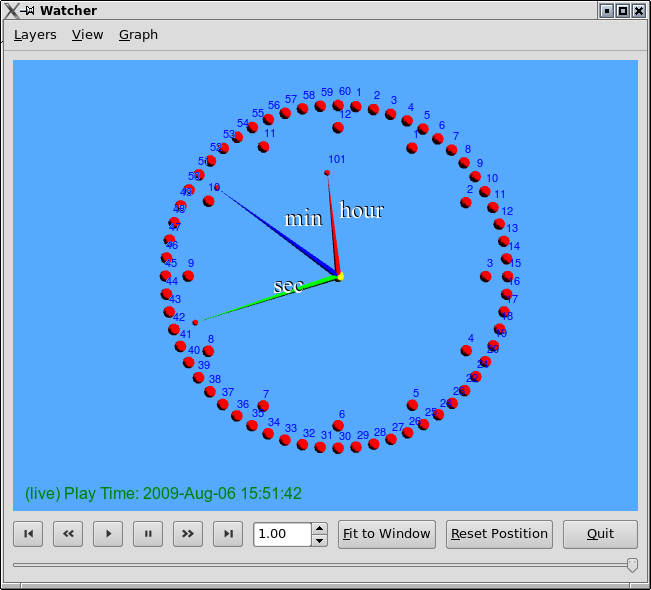
\includegraphics[width=0.8\textwidth]{legWatcherGUI.eps}
\caption{The legacy watcher showing a running instance of showClock.}
\label{fig:LegacyWatcherClock}
\end{figure}

\subsubsection{Command Line Options}
\begin{itemize}
\item {\tt -h} or {\tt --help}, show a usage message and exit. 
\item {\tt -f} of {--configFile}, gives the location of the configuration file. If not given a default one will be created, used, and saved on program exit.
\end{itemize}

\subsubsection{Configuration}
\begin{itemize}
\item {\tt server}, name or ipaddress of the server to connect to.
\item {\tt service}, name of service (usaully "watcherd") or port number on which the server is listening.
\item {\tt layers}, a listing of layers from the Layers menu. All layers the watcher knows about will show up here in a {\tt layername = bool} pair. 
If the bool is {\tt true}, the layer will be active (and shown), if {\tt false} the layer will not be shown. Every {\tt layername} will become
an entry in the {\tt layers} menu in the GUI.
\item {\tt nodes3d = bool}, if {\tt boolval} is {\tt true}, the GUI will use 3d shapes to diplay the MANET elements, otherwise 2d shapes will be used.
\item {\tt monochrome = bool}, if {\tt bool} is true all GUI elements in the main window will be black and white. Otherwise colors will be used. 
\item {\tt displayBackgroundImage = bool}, if {\tt bool} is true and a background image file is given, the background will be displayed. Otherwise it will not.
\item {\tt showVerboseStatusString = false}, if {\tt true} show extra debugging information in the status string in the main window.
\item {\tt showWallTime = true}, if {\tt true} show the current system time in the status string in the main window.
\item {\tt showPlaybackTime = true}, if {\tt true} show the current playback time (when the events happened) in the status string in the main window.
\item {\tt showPlaybackRange = true}, if {\tt true} show total time range (first event, last event) of playback in the status string in the main window.
\item {\tt statusFontName = ``name''}, the font name of the status string in the main window. e.g. ``Helvetica''. 
\item {\tt scaleText = float}, how much to scale the text in the main window.
\item {\tt scaleLine = float}, how much to scale lines in the main window.
\item {\tt layerPadding = float}, how much padding (in pixels) to place between layers. 
\item {\tt gpsScale = float}, a constant to multiply GPS coordinates against.
\item {\tt antennaRadius = float}, how big the ``antenna radius'' is in meters (for display only - does not effect connectivity). 
\item {\tt ghostLayerTransparency = float}, how transparent to make the ``ghost layer'', when layers are spread more than a few pixels apart.
\item {\tt statusFontPointSize = float}, the font size of the status string. 
\item {\tt backgroundImage:imageFile=filename}, the location of the background image to use, or ``none'' (with quotes) if not using a background image.
\item {\tt backgroundImage:coordinates = [ x, width, y, height]}, the initial location of the background image. This can be adjusted manually by using the right mouse button, while holding the shift key.
\item {\tt viewPoint : angle = [x, y, z]}, the initial angle of the main window view point with respect to the MANET.
\item {\tt viewPoint : scale = [x, y, z]}, the initial scale of the main window view point with respect to the MANET.
\item {\tt viewPoint : shift = [x, y, z]}, the initial shift of the main window view point with respect to the MANET.
\item {\tt backgroundColor : r=float}, the {\it red} component of the background color expressed as number between 0 and 1.
\item {\tt backgroundColor : g=float}, the {\it green} component of the background color expressed as number between 0 and 1.
\item {\tt backgroundColor : b=float}, the {\it blue} component of the background color expressed as number between 0 and 1.
\item {\tt backgroundColor : a=float}, the {\it alpha} component of the background color expressed as number between 0 and 1.
\end{itemize}

\subsubsection{User Interface}
The user interface for the watcher consists of a main window which displays the MANET, playback controls, a few buttons, and three pull down menus.

The main window is the heart of the visualization of the MANET. It is here where all the nodes, connections, labels, and layers are displayed. The 
user can use interact with the main window via the mouse or keyboard shortcuts. Mouse usage and keyboard shortcuts are given below.

\subsubsection{Layer Menu}
\begin{figure}[htb]
\centering
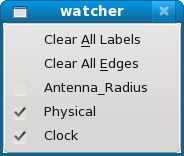
\includegraphics[width=0.2\textwidth]{legWatcherLayersMenu.eps}
\caption{An instance of the layer menu in the watcher GUI. Layers appear here dynamically.}
\label{fig:legWatcherLayersMenu}
\end{figure}

\subsubsection{View Menu}
\begin{figure}[htb]
\centering
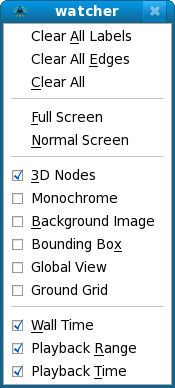
\includegraphics[width=0.2\textwidth]{legWatcherViewMenu.eps}
\caption{The view menu in the watcher GUI.}
\label{fig:legWatcherViewMenu}
\end{figure}

\subsubsection{Graph Menu}





\subsection{ogreWatcher}

Grr! Arg!

\begin{figure}
\centering
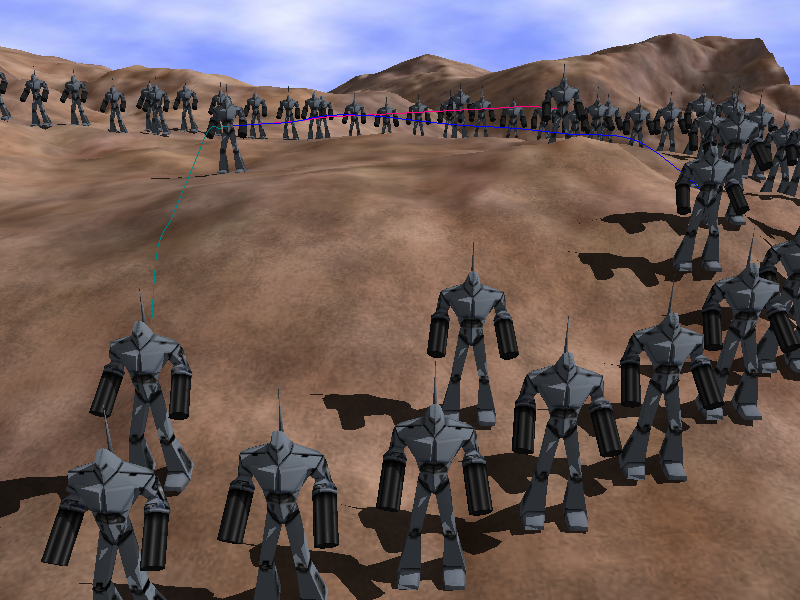
\includegraphics[width=0.8\textwidth]{ogreWatcherGUI.eps}
\caption{The ogreWatcher showing a running instance of showClock.}
\label{ogreWatcher}
\end{figure}

Built with OGRE.

\subsubsection{Configuration}

\begin{itemize}
\item {\tt -h} or {\tt --help}, show a usage message and exit. 
\item {\tt -c configfile}, gives the location of the configuration file. If not given a default one will be created, used, and saved on program exit.
\end{itemize}

\subsubsection{Command Line Options}

\begin{itemize}
\item {\tt server}, name or ipaddress of the server to connect to.
\item {\tt service}, name of service (usaully "watcherd") or port number on which the server is listening.
\end{itemize}

\subsection{Watcher3d}
Built with Delta-3d.


\subsection{messageStream2Text}

{\it messageStream2Text} is not your typical GUI in that it has no graphical interface. It's in the GUI section though as it uses 
the GUI watcher API to talk to a running watcher daemon. It was written (and is used) as a tool to debug the message stream interface. It simply
connects to a daemon instance, requests a message stream, and dumps all the recieved messages to the console on stdout. Think of it as a 
tcpdump for watcher message streams. 

{\it messageStream2Text} source code can be found in {\tt .\slash src\slash clients\slash messageStream2Text}. 

\subsubsection{Configuration}

\begin{itemize}
\item {\tt -h} or {\tt --help}, show a usage message and exit. 
\item {\tt -c configfile}, gives the location of the configuration file. If not given a default one will be created, used, and saved on program exit.
\end{itemize}

\subsubsection{Command Line Options}

\begin{itemize}
\item {\tt server}, name or ipaddress of the server to connect to.
\item {\tt service}, name of service (usaully "watcherd") or port number on which the server is listening.
\end{itemize}


\subsection{Earth Watcher}
\label{EarthWatcher}

The Earth Watcher is a daemon application for Linux systems that allows
visualization of Watcher events in the Google Earth GUI.

{\it earthWatcher} source code can be found in {\tt .\slash src\slash
clients\slash earthWatcher}. The binary produced after building is 
named {\tt earthWatcher}. 

\subsubsection{Command Line Options}
\begin{itemize}
\item {\tt -h} or {\tt --help}, show a usage message and exit. 
\item {\tt -c} of {--configFile}, gives the location of the configuration file. If not given a default one will be created, used, and saved on program exit.

\item {\tt -a} or {\tt --latoff}, translate GPS coordinates relative to a given latitude
\item {\tt -A} or {\tt --altoff}, translate GPS coordinates relative to the given altitude
\item {\tt -c} or {\tt --config}, specify a configuration file (default:
earthWatcher.cfg)
\item {\tt -d} or {\tt --speed}, specify the event playback rate
\item {\tt -h} or {\tt --help}, display this help message
\item {\tt -i} or {\tt --icon-scale}, adjust the size of node icons
\item {\tt -I} or {\tt --icon-path}, specify the node icon to use
\item {\tt -o} or {\tt --output}, specifies the output KML file
\item {\tt -O} or {\tt --lonoff}, translate GPS coordinates relative to a given longitude
\item {\tt -r} or {\tt --refresh}, write the the output every SECS seconds
\item {\tt -s} or {\tt --server}, connect to the watcher server on the given host
\item {\tt -S} or {\tt --seek}, start event playback at the specified timestamp.  May be specified relative to the first and last timestamps in the Watcher database by prefixing the offset with "+" or "-". Example: +5000 means 5 seconds after the first event in the database.
\item{\tt  -t} or {\tt --steps}, number of points to use when drawing a spline (default: 2)

\end{itemize}

\subsubsection{Configuration}
\begin{itemize}
\item {\tt server}, name or ipaddress of the server to connect to.
\item {\tt service}, name of service (usaully "watcherd") or port number on which the server is listening.
\item {\tt layers}, a listing of layers from the Layers menu. All layers the watcher knows about will show up here in a {\tt layername = bool} pair. 
If the bool is {\tt true}, the layer will be active (and shown), if {\tt false} the layer will not be shown. Every {\tt layername} will become
a folder in the {\tt Places} menu in the Google Earth GUI.
\item {\tt layerPadding = float}, how much padding (in feet) to place between layers. 
\item {\tt latOff = float}, translate GPS coordinates relative to a given latitude.
\item {\tt lonOff = float}, translate GPS coordinates relative to a given longitude.
\item {\tt outputFile = string}, specifies the output KML file.
\item {\tt iconPath = string}, specify an alternate icon to use for nodes.
\item {\tt splineSteps}, the number of points in a spline when drawing edges.
\end{itemize}

\subsubsection{Reloading Configuration File}

EarthWatcher checks for changes in the configuration file while running.  The purpose of this feature is to allow for
defined layers to be toggled on or off during runtime.  No options other than the layers are checked for changes during runtime.

\subsubsection{Translating GPS coordinates}

If the GPS coordinates stored in the Watcher database during a test run are not
accurate, the EarthWatcher has options to translate the coordinates relative to
some location on the Earth.  For example, the origin is located in the Atlantic
Ocean off the coast of West Africa.  Using the {\tt latOff} and {\tt lonOff}
options can place the nodes in a more geographically interesting location.


\printindex
\end{document}
